%%%%%%%%%%%%%%%%%%%%%%%%%%%%%%%%%%%%%%%%%%%%%%%%%%%%%%%%%%%%%%%%%%%%%%%%
%    INSTITUTE OF PHYSICS PUBLISHING                                   %
%                                                                      %
%   `Preparing an article for publication in an Institute of Physics   %
%    Publishing journal using LaTeX'                                   %
%                                                                      %
%    LaTeX source code `ioplau2e.tex' used to generate `author         %
%    guidelines', the documentation explaining and demonstrating use   %
%    of the Institute of Physics Publishing LaTeX preprint files       %
%    `iopart.cls, iopart12.clo and iopart10.clo'.                      %
%                                                                      %
%    `ioplau2e.tex' itself uses LaTeX with `iopart.cls'                %
%                                                                      %
%%%%%%%%%%%%%%%%%%%%%%%%%%%%%%%%%%
%
%
% First we have a character check
%
% ! exclamation mark    " double quote  
% # hash                ` opening quote (grave)
% & ampersand           ' closing quote (acute)
% $ dollar              % percent       
% ( open parenthesis    ) close paren.  
% - hyphen              = equals sign
% | vertical bar        ~ tilde         
% @ at sign             _ underscore
% { open curly brace    } close curly   
% [ open square         ] close square bracket
% + plus sign           ; semi-colon    
% * asterisk            : colon
% < open angle bracket  > close angle   
% , comma               . full stop
% ? question mark       / forward slash 
% \ backslash           ^ circumflex
%
% ABCDEFGHIJKLMNOPQRSTUVWXYZ 
% abcdefghijklmnopqrstuvwxyz 
% 1234567890
%
%%%%%%%%%%%%%%%%%%%%%%%%%%%%%%%%%%%%%%%%%%%%%%%%%%%%%%%%%%%%%%%%%%%
%
\documentclass[12pt]{iopart}
\newcommand{\gguide}{{\it Preparing graphics for IOP Publishing journals}}
%Uncomment next line if AMS fonts required
%\usepackage{iopams}  
%
%% My own packages
%
\usepackage{ dsfont }
\usepackage{hyperref}
\usepackage{graphicx}
%
%% User-defined commands
%
\newcommand{\ddt}[1]{\frac{d #1}{dt}}
%\newcommand{\hmone}[1]{\|#1\|_{H^{-1}}}
\newcommand{\hmone}[1]{\|\nabla^{-1} #1\|_{L^{2}}}
\newcommand{\ltwo}[1]{\|#1\|_{L^{2}}}
%\newcommand{\hone}[1]{\|#1\|_{H^{1}}}
\newcommand{\hone}[1]{\| \nabla #1\|_{L^{2}}}
\newcommand{\htwo}[1]{\|#1\|_{H^{2}}}
\newcommand{\sint}[1]{\int_{D} #1 \, d^{d}\mathbf{x}}
\newcommand{\tint}[1]{\int_{0}^{T} #1 \, dt}
\renewcommand{\vec}[1]{\mathbf{#1}}
\newcommand{\linf}[1]{\| #1 \|_{L^{\infty}}}
\newcommand{\tavg}[1]{\langle  #1 \rangle}
\renewcommand{\u}{\mathbf{u}}
%\newcommand{\ppt}[1]{\frac{\partial #1}{\partial t}}
\newcommand{\ppt}[1]{\partial_{t} #1}
\newcommand{\lap}{\Delta }
\newcommand{\invlap}{\Delta^{-1}}
%\newcommand{\lap}{\nabla^{2}}
%\newcommand{\invlap}{\nabla^{-2}}
\newcommand{\pbrac}[1]{\left( #1 \right)}
\newcommand{\sbrac}[1]{\left[ #1 \right]}
\newtheorem{lemma}{Lemma}
\newtheorem{corollary}{Corollary}

\begin{document}

\title[Diffusion-limited mixing by incompressible flows]{Diffusion-limited mixing by incompressible flows}

\author{C J Miles$^{1,2,3}$ and C R Doering$^{1,2,3}$ }

\address{$^1$ Department of Physics, University of Michigan,
Ann Arbor, MI 48104-1040, USA}
\address{$^2$ Department of Mathematics, University of Michigan,
Ann Arbor, MI 48104-1043, USA}
\address{$^3$ Center for the Study of Complex Systems, University of Michigan,
Ann Arbor, MI 48104-1107, USA}
\ead{doering@umich.edu}
\vspace{10pt}
\begin{indented}
\item[]February 2014
\end{indented}

\begin{abstract}
Incompressible flows can be effective mixers by appropriately advecting a passive tracer to produce small filamentation length scales. The Batchelor length scale \cite{Batchelor1959a} was proposed as the lower limit of length scales achievable in turbulent flows. Here, we provide numerical evidence that this limitation may be even more general, applying as well to all incompressible flows under mild physical constraints such as bounded enstrophy or energy. We consider local-in-time flow optimisation under these flow intensity constraints with the objective of maximising mixing rate performance. We observe that, for enstrophy-bounded optimal flows, the strength of diffusion has no impact on the long-term mixing rate performance. For energy-constrained optimal flows, however an increase in the strength of diffusion decreases the mixing rate. We provide analytical lower bounds on mixing rates and length scales achievable under related constraints (point-wise bounded speed and rate-of-strain) by extending the work of \cite{JFM2011} and \cite{Chi-Cheu1996}. 

\end{abstract}
%
\pacs{47.85.lk, 47.85.L-, 42.10, 47.57.eb}
\ams{76R50, 37A25, 76F25, 76D55}
%
% Uncomment for keywords
\vspace{2pc}
\noindent{\it Keywords}: Mixing, incompressible flow, diffusion processes, flow control and optimisation, Batchelor scale

% Uncomment for Submitted to journal title message
\submitto{\NL}
%
% Uncomment if a separate title page is required
%\maketitle
% 
% For two-column output uncomment the next line and choose [10pt] rather than [12pt] in the \documentclass declaration
%\ioptwocol
%

\section{Introduction}

Mixing a passive tracer concentration via an incompressible fluid flow is important to many areas of science and engineering. A question of interest across these domains is ``How can one stir to enhance the rate of mixing?'' We explore this question and study the impact of molecular diffusion. We address this topic by considering an incompressible flow with mild physical constraints in a periodic box with side length $L$ in $d$ dimensions. We consider a mean-zero tracer concentration field $\theta$ that evolves according to the advection-diffusion equation,
\begin{equation}
	\label{eq:PDE_advection}
	\ppt{\theta}+\mathbf{u}\cdot \nabla \theta=\kappa \lap\theta,
\end{equation}
with initial data $\theta(\mathbf{x},0)=\theta_{0}(\mathbf{x})$, where $\kappa$ is the molecular diffusion coefficient and $\mathbf{u}(\mathbf{x},t)$ is a incompressible ($\nabla\,\cdot\, \vec{u}=0$) flow field. The flow is constrained by enstrophy $\ltwo{\nabla\u} = \Gamma L^{d/2}$ or energy $\ltwo{\u} = UL^{d/2}$ where $\Gamma$ is the root mean square rate-of-strain and $U$ is the root mean square speed. We primarily use the $H^{-1}$ norm or mix-norm throughout to measure homogenisation,   

\begin{equation}
\hmone{\theta}=\sqrt{\sint{ |\nabla^{-1} \theta( \vec{x},t)|^2}}=\sqrt{ \sum_{\vec{k}\neq \vec{0}} L^d \frac{|\hat{\theta}_{\vec{k}}(t)|^{2}}{|\vec{k}|^2}}
\end{equation}
where $\nabla^{-1}=\nabla \Delta^{-1}$, the operator $\Delta^{-1}$ acting on  a function $\rho$ returns the solution $\phi$ of the Poisson equation $ \Delta \phi = \rho $, and $\hat{\theta}_{\vec{k}}(t) =  \frac{1}{L^{d}}\sint{\theta(\vec{x},t)e^{-i\vec{k}\cdot\vec{x}}}$.  Lower values of the  $H^{-1}$ norm corresponds to a more mixed state. Note that $H^{-1}$ norm can decrease in two ways: either by decreasing the amplitudes of $|\hat{\theta}_{\vec{k}}|$ or by advecting the flow such that the tracer concentration acquires more spectral mass in the higher wave numbers and takes advantage of the $1/|\vec{k}|^2$ dependence. We use the $H^{-1}$ norm to define the (exponential) rate of mixing as
\begin{equation}
\label{eq:rate}
r(t) = -  \frac{\ddt{}\hmone{\theta}}{\hmone{\theta}}.
\end{equation}
The $L^{2}$ norm $\ltwo{\theta}$ and the $H^{1}$ norm $\hone{\theta}$ are also common measures of mixing and will be considered here as well. 

We define the following ratio as a measure of the characteristic filamentation length scale:
\begin{equation}
\lambda(t)\equiv  2\pi \frac{\|\nabla^{-1}\theta(\,\cdot\,,t)\|_{L^{2}}}{\|\theta(\,\cdot\,,t)\|_{L^{2}}}.
\end{equation}
Note that $\lambda(t)$ returns the wavelength of the wave number $\vec{k}$ for a tracer concentration field composed only of the Fourier mode with wave number $\vec{k}$ (i.e. $\theta(\vec{x},t) = Re[ A e^{-i\vec{k}\cdot \vec{x}}]$ where $A$ is a complex constant). In general, $\lambda$ is the weighted root mean square wavelength with weights given by $|\theta_{\vec{k}}|/\ltwo{\theta}$. 


For the enstrophy-bounded flow problem, we choose the same length scale $L$, the velocity scale $L\Gamma $, and  the time scale $1/\Gamma$. For the energy-bounded flow problem, we non-dimensionalise the system by choosing $L$ as the length scale, $U$ as the velocity scale, and $L/U$ as the time scale.  Both scalings produce the following form of the advection-diffusion equation,
\begin{equation}
\label{eq:nd_ade}
	\ppt{\theta}+\mathbf{u}\cdot \nabla \theta=\frac{1}{Pe} \lap\theta,
\end{equation}
where $Pe=  \frac{\Gamma L^2}{\kappa}$ for the enstrophy-constrained case and $Pe= \frac{UL}{\kappa}$ for the energy-constrained case.   The constraints on the flow become $\ltwo{\nabla\u} = 1$ or $\ltwo{\u} = 1$.



We will first review results for the $Pe = \infty$ enstrophy-constrained case. \cite{JFM2011} showed numerical evidence that the filament width $\lambda$ seemingly decreased continually by instantaneous flow optimisation. This type of optimisation will be considered in this work as well. Self-similar flows can realise a decreasing $\lambda$ over time as shown analytically by \cite{Alberti2014a}.  It was rigorously proven independently by \cite{GI2014} and \cite{CS2013} that $\lambda$ decreased at most exponentially --- consistent with \cite{JFM2011}  and \cite{Alberti2014a}. The work of \cite{GI2014} relied on PDE regularisation results of \cite{Crippa} while the approach of \cite{CS2013} used methods from optimal transportation theory \cite{villani2003topics}.

For $Pe = \infty$ energy-constrained problem, \cite{JMP2012} showed that a `chequerboard' flow can also provide continually decreasing length scales. Moreover, $\lambda$ decreased at a fast enough rate to approach zero in finite time in contrast to the enstrophy-constrained problem where $\lambda$ decreases to zero in infinite time.

The inclusion of diffusion ($Pe <\infty$) with the objective of optimal mixing has been explored.  \cite{DF2014} investigated optimal mixing and study the evolution of the mentioned measures ($H^{-1}, L^2,$ and $H^1$ norms) of mixing under the chequerboard flow introduced by \cite{JMP2012}. They show that the $H^{-1}$ and $L^2$ norms decrease monotonically under this flow while the $H^{1}$ increases until it reaches a peak and then decreases. This peak corresponds to a  time when the length scales developed are small enough for diffusion to effectively act on steep gradients. \cite{Miles2017a} explored this phenomena further in the context of a shell model, a reduced model using ordinary differential equations that mimic the spectral dynamics of the advection-diffusion equation. The authors concluded that shell-model mixing could not surpass length scales given by $\sqrt{\kappa/ \Gamma}$ for enstrophy-constrained flows and $\kappa/U$ for energy-constrained flows up to $O(1)$ constants. These length scales can be identified as a generalised Batchelor scale \cite{Batchelor1959a}, introduced in the context of turbulence theory. 
 
 
In this work, we explore how diffusion impacts the evolution of the filament width $\lambda$ over time and mixing rates. We show numerical evidence that $\lambda$ appears to be limited by the Batchelor scale as seen in the shell model. Even when actively trying to choose the most optimal flow to minimise filamentation length. Thus, this may suggest that the Batchelor scale does not only limit turbulent flows but also all incompressible flows under the flow constraints considered here. Although these quantities have been known in the context of turbulence theory, the impact of these limitations on mixing rates has not been fully studied to our knowledge.

Furthermore, we believe that the study of determining the smallest length scales achievable demands more attention. This assumption is used today throughout the computational fluid dynamics community to provide a heuristic for the grid resolutions necessary. Thus, it is important to determine what conditions on $\mathbf{u}$ are necessary to justify this assumption. 

The paper is organised as follows. We introduce the necessary theory regarding local-in-time optimisation, a shell model, and $L^{\infty}$ flow constraints in section \ref{sec:theory}. Section \ref{sec:numerical_experiment} details the methodology and results of numerically implementing local-in-time flow optimisation. Lastly, we finish with a discussion and conclusion in sections \ref{sec:discussion} and \ref{sec:conclusion} respectively.

\section{Theory}
\label{sec:theory}
\subsection{Local-in-time optimisation}
We consider the local-in-time optimisation strategy first introduced by \cite{JFM2011} in the diffusion-less case. We find that this strategy generalises to the case with diffusion. The local-in-time optimal velocity fields maximise the instantaneous mixing rate by minimising $\ddt{}\hmone{\theta}^2$ or equivalently minimising $\ddt{\lambda^2}$ . The optimal velocity fields are given instantaneously by (in non-dimensional form)
%
\begin{equation}
\mathbf{u}= \frac{\mathds{P}(\theta \nabla \invlap\theta)}{\langle |\mathds{P}(\theta \nabla \invlap\theta)|^2\rangle^{1/2}}
\end{equation} 
%
for the energy constraint and by 
%
\begin{equation}
\mathbf{u}= \frac{-\invlap\mathds{P}(\theta \nabla \invlap\theta)}{\langle |\nabla^{-1}\mathds{P}(\theta \nabla \invlap\theta)|^2\rangle^{1/2}}
\end{equation}
%
for the enstrophy constraint where $\mathds{P}$ is the Leray divergence-free projector given by $\mathds{P}(\vec{v}) = \vec{v} - \nabla \Delta^{-1}(\nabla \cdot \vec{v})$. These flows will be studied numerically later and is the main focus of this paper.


\subsection{Shell model predictions of local-in-time optimisation}

The shell model is a reduced model of the spectral dynamics present in the advection-diffusion equation. The model consists of a system of ordinary differential equations with nearest-neighbour coupling between `shells' in wave number space. \cite{Miles2017a} performed local-in-time mixing optimisation in this model. The shell-model analysis predicts a limiting length scale given by the Batchelor scale, $\Lambda_{\Gamma} =\sqrt{\frac{\kappa}{\Gamma}}$  and its generalisation $\Lambda_{U}= \frac{U}{\kappa} $. The non-dimensional versions are given by $\lambda_{\Gamma}= \frac{1}{\sqrt{Pe}}$ and $\lambda_{U} = \frac{1}{Pe}$.  Also from here forward, we will refer to the Batchelor scale to mean either $\lambda_{\Gamma}$ or its generalisation $\lambda_{U}$.  The predicted long-term rates (after reaching the Batchelor scale) are given by $R_{\Gamma} =\kappa/\lambda_{\Gamma}^2 $  and  $R_{U}=\kappa/\lambda_{U}^2$  The non-dimensional versions are given by $r_{\Gamma} =1$ and $r_{U} = Pe $.

\subsection{Bounds for $L^{\infty}$ constrained flows}
We consider a subset of $L^{2}$ constrained flows --- those belonging to $L^{\infty}$. In this restricted setting the rate-of-strain and speed are bounded point-wise uniformly in space and time rather than demanding that they merely be $L^2$ integrable as before. We will provide bounds on $\lambda$ and measures of mixing in this restricted setting. 

\label{sec:linfty_flows}
\subsubsection{Results for $\linf{\nabla \vec{u}} = 1$}

The time derivative of $\lambda^2$ is
%
\begin{equation}
	\ddt{\lambda^2} = \frac{2}{Pe}
		\left[ 
			\frac{\hone{\theta}^2\hmone{\theta}^2}
					{\ltwo{\theta}^4}  
			- 1
		\right]
		+ 2 \frac{\sint{\nabla^{-1}\theta \cdot \nabla\vec{u} \cdot 
							\nabla^{-1}\theta  }}
					  {\ltwo{\theta}^{2}}
\end{equation}
and by H\"older's inequality, we deduce
\begin{equation}
\label{eq:length_ineq_rate-of-strain}
	\ddt{\lambda^2} \geq \frac{2}{Pe} \left[ 
			\frac{\hone{\theta}^2\hmone{\theta}^2}
					{\ltwo{\theta}^4}  
			- 1
		\right] - 2  \lambda^2 .
\end{equation}
This establishes a lower bound on $\lambda$ at each instant: by apply Gr\"onwall's inequality and the fact that the bracketed term is greater than or equal to zero, it follows that
%
\begin{equation}
\label{eq:exponential_enstrophy}
	\lambda (t) \geq \lambda(0)e^{- t}.
\end{equation}
%
Therefore, perfect mixing in finite time is impossible for bounded rate-of-strain flows.

Furthermore,
%
\numparts \begin{eqnarray}
\frac{d}{dt}\left(\frac{\|\nabla\theta\|_{L^{2}}^2}{\|\theta\|_{L^{2}}^2}\right) &= \frac{\|\theta\|_{L^{2}}^2\frac{d}{dt}\|\nabla\theta\|_{L^{2}}^2-\|\nabla\theta\|_{L^{2}}^2\frac{d}{dt}\|\theta\|_{L^{2}}^2}{\|\theta\|_{L^{2}}^4}\\
&= \frac{-2\int \partial_{i}u_{j}\partial_{i}\theta\partial_{j}\theta - \frac{2}{Pe} \|\Delta\theta\|_{L^{2}}^2}{\|\theta\|_{L^{2}}^2}+\frac{2}{Pe}\frac{\|\nabla\theta\|_{L^{2}}^4}{\|\theta\|_{L^{2}}^4} \\
&=-\frac{2}{Pe}\left(\frac{\|\Delta\theta\|_{L^{2}}^2}{\|\theta\|_{L^{2}}^2} - \frac{\|\nabla\theta\|_{L^{2}}^4}{\|\theta\|_{L^{2}}^4} \right) - 2\frac{\sint{\nabla\theta \cdot \nabla\vec{u} \cdot 
							\nabla\theta  }}{\|\theta\|_{L^{2}}^2} 
\\
&\leq 2 \frac{\hone{\theta}^2}{\ltwo{\theta}^2}
\end{eqnarray} \endnumparts
%
and using $\ddt{}\ltwo{\theta}^2 = -\frac{2}{Pe} \hone{\theta}^2$, it follows that
\begin{equation}
\ltwo{\theta}\geq  \ltwo{\theta_{0}}\exp\left[-\frac{1}{2Pe}\frac{\hone{\theta_{0}}^2}{\ltwo{\theta_{0}}^2}\left(e^{2 t} -1\right)\right].
\end{equation}
Using this with (\ref{eq:exponential_enstrophy}), we deduce the lower bound
\begin{equation}
\hmone{\theta} \geq  \hmone{\theta_{0}} \exp\left[- t -\frac{1}{2 Pe}\frac{\hone{\theta_{0}}^2}{\ltwo{\theta_{0}}}\left(e^{2 t} -1\right)\right].
\end{equation}

\subsubsection{Results for $\linf{\u}= 1$}
Here we extend the result of \cite{Chi-Cheu1996} to show that the presence of diffusion rules out perfect mixing in finite time for bounded velocity flows.  First note that
%
\begin{eqnarray}
	 \hone{\theta}^2 &=& - 2\sint{\theta \lap \theta} \\
	 							&=& Pe \sint{\theta\left(\ppt{\theta}
	 									-\frac{1}{Pe}\lap \theta\right)} 
	 									-Pe \sint{\theta\left(\ppt{\theta}
	 									+\frac{1}{Pe}\lap \theta\right)} 
\end{eqnarray},
%
\begin{eqnarray}
	\ddt{}\ltwo{\theta}^2 &=& 2\sint{\theta\ppt{\theta}} \\
										 &=&\sint{\theta\left(\ppt{\theta}
	 									-\frac{1}{Pe}\lap \theta\right)} 
										 + \sint{\theta\left(\ppt{\theta}
	 									+\frac{1}{Pe}\lap \theta\right)} 
\end{eqnarray},
%
and
%
\begin{eqnarray}
	\ddt{}\hone{\theta}^2 &=& -2\sint{\ppt{\theta}\lap \theta} \\
	 									&=& Pe \sint{\left(\ppt{\theta}
	 									-\frac{1}{Pe}\lap \theta\right)^2} 
	 									-Pe \sint{\left(\ppt{\theta}
	 									+\frac{1}{Pe}\lap \theta\right)^2} .
\end{eqnarray}

Then compute:
%
\begin{eqnarray*}
	\ddt{} \pbrac{ \frac{\hone{\theta}^2}{\ltwo{\theta}^2} } 
			&=& \frac{1}{\ltwo{\theta}^4}
			\sbrac{
				\ltwo{\theta}^2\ddt{}\hone{\theta}^2
				-\ddt{}\ltwo{\theta}^2\hone{\theta}^2			
			}\\
			&=& \frac{1}{\ltwo{\theta}^4}
			\sbrac{
				\ltwo{\theta}^2
				\pbrac{
					Pe \sint{\left(\ppt{\theta}
	 									-\frac{1}{Pe}\lap \theta\right)^2} 
 					-Pe\sint{\left(\ppt{\theta}
	 									+\frac{1}{Pe}\lap \theta\right)^2} 
				}
			}\\
		&-&\frac{1}{\ltwo{\theta}^4}
			\sbrac{
				Pe
				\pbrac{
					 \sint{\theta\left(\ppt{\theta}
	 									-\frac{1}{Pe}\lap \theta\right)} 
 				}^2		
 				-
 				Pe
 				\pbrac{
					 \sint{\theta\left(\ppt{\theta}
	 									+\frac{1}{Pe}\lap \theta\right)} 
 				}^2					
			}.
\end{eqnarray*}
%
Using H\"older's inequality and (\ref{eq:PDE_advection}), this simplifies to
%
\begin{eqnarray*}
	\ddt{} \pbrac{ \frac{\hone{\theta}^2}{\ltwo{\theta}^2} } 
			&\leq & \frac{Pe}{\ltwo{\theta}^2}
			\sbrac{
					 \sint{(\vec{u}\cdot \nabla \theta)^2} 
			}.
\end{eqnarray*}
Again applying H\"older's inequality we have
\begin{equation}
\label{eq:k2growth_energy}
	\ddt{} 
		\pbrac{ 
			\frac{\hone{\theta}^2}{\ltwo{\theta}^2} 
		} 
		\leq  
		Pe
		\frac{\hone{\theta}^2}{\ltwo{\theta}^2} 
\end{equation}
%
and thus 
%
\begin{equation}
		\frac{\hone{\theta}}{\ltwo{\theta}} 
		\leq  
		\frac{\hone{\theta_0}}{\ltwo{\theta_0}}
		\exp{\pbrac{\frac{Pe}{2} t}}.
\end{equation}
%
The inequality $\hone{\theta}\hmone{\theta}\geq \ltwo{\theta}^2$ then ensures that
%
\begin{equation}
\label{eq:lambda_bound}
\lambda(t) \geq \frac{\ltwo{\theta_0}}{\hone{\theta_0}}\exp{\pbrac{-\frac{Pe}{2}t}}.
\end{equation}
%
Using (\ref{eq:k2growth_energy}) together with  $\ddt{}\ltwo{\theta}^2 = -\frac{2}{Pe} \hone{\theta}^2$ we observe that
%
\begin{equation}
\ltwo{\theta}\geq \ltwo{\theta_{0}}\exp\left[-\frac{1}{Pe^2}\frac{\hone{\theta_0}^2}{\ltwo{\theta_0}^2}\left(e^{Pe \, \, t}-1\right)\right]
\end{equation}
%
and this combined with  (\ref{eq:lambda_bound}) implies
%
\begin{equation}
\hmone{\theta}\geq \frac{\ltwo{\theta_{0}}^2}{\hone{\theta_0}}\exp\left[-\frac{Pe}{2} \,\, t-\frac{1}{Pe^2}\frac{\hone{\theta_0}^2}{\ltwo{\theta_0}^2}\left(e^{Pe \,\, t}-1\right)\right].
\end{equation}



%
\section{Numerical experiment: local-in-time optimisation}
\label{sec:numerical_experiment}
\subsection{Methodology}

We solve (\ref{eq:nd_ade}) by using a Fourier basis to represent the $512 \times 512$ discretised spatial domain with a 4th order Runge-Kutta time-stepping method. All simulation code was created in the programming language Python with package modules, pyfftw and numpy. The code repository can be found at \href{http://github.com/cjm715/lit}{ http://github.com/cjm715/lit}.

\subsection{Results}

\begin{figure}
\includegraphics[width=\textwidth]{images/enstrophy_film}
\caption{Local-in-time optimisation with enstrophy constraint. Top filmstrip is for $Pe =\infty$ and the bottom filmstrip is $Pe=256$. Note that the grey-scale for the $Pe=\infty$ is constant in time while it is adjusted to show the tracer concentration structure in the finite $Pe$ case. }
\label{fig:enstrophy_film}
\end{figure}
%
\begin{figure}
\includegraphics[width=\textwidth]{images/energy_film}
\caption{Local-in-time optimisation with energy constraint. Top filmstrip is for $Pe = \infty$ and the bottom filmstrip is $Pe=32$. Note that the grey-scale for the $Pe=\infty$ is constant in time while it is adjusted to show the tracer concentration structure in the finite $Pe$ case. }
\label{fig:energy_film}
\end{figure}
%
\begin{figure}
\includegraphics[width=\textwidth]{images/enstrophy_norms}
\caption{$H^{-1}, L^{2},$ and $H^{1}$ norms of the concentration field under the optimal enstrophy-constrained flow.  }
\label{fig:enstrophy_norms}
\end{figure}
%
\begin{figure}
\includegraphics[width=\textwidth]{images/energy_norms}
\caption{$H^{-1}, L^{2},$ and $H^{1}$ norms of the concentration field under the optimal energy-constrained flow.}
\label{fig:energy_norms}
\end{figure}
%
\begin{figure}
\includegraphics[width=\textwidth]{images/enstrophy_length}
\caption{The left subplot shows the filament length $\lambda$ over time subject to the optimal enstrophy-constrained flow. The right subplot is the same data except scaled: $\lambda(t)/\lambda_{\Gamma} = \lambda(t)\sqrt{Pe}$.}
\label{fig:enstrophy_length}
\end{figure}
%
\begin{figure}
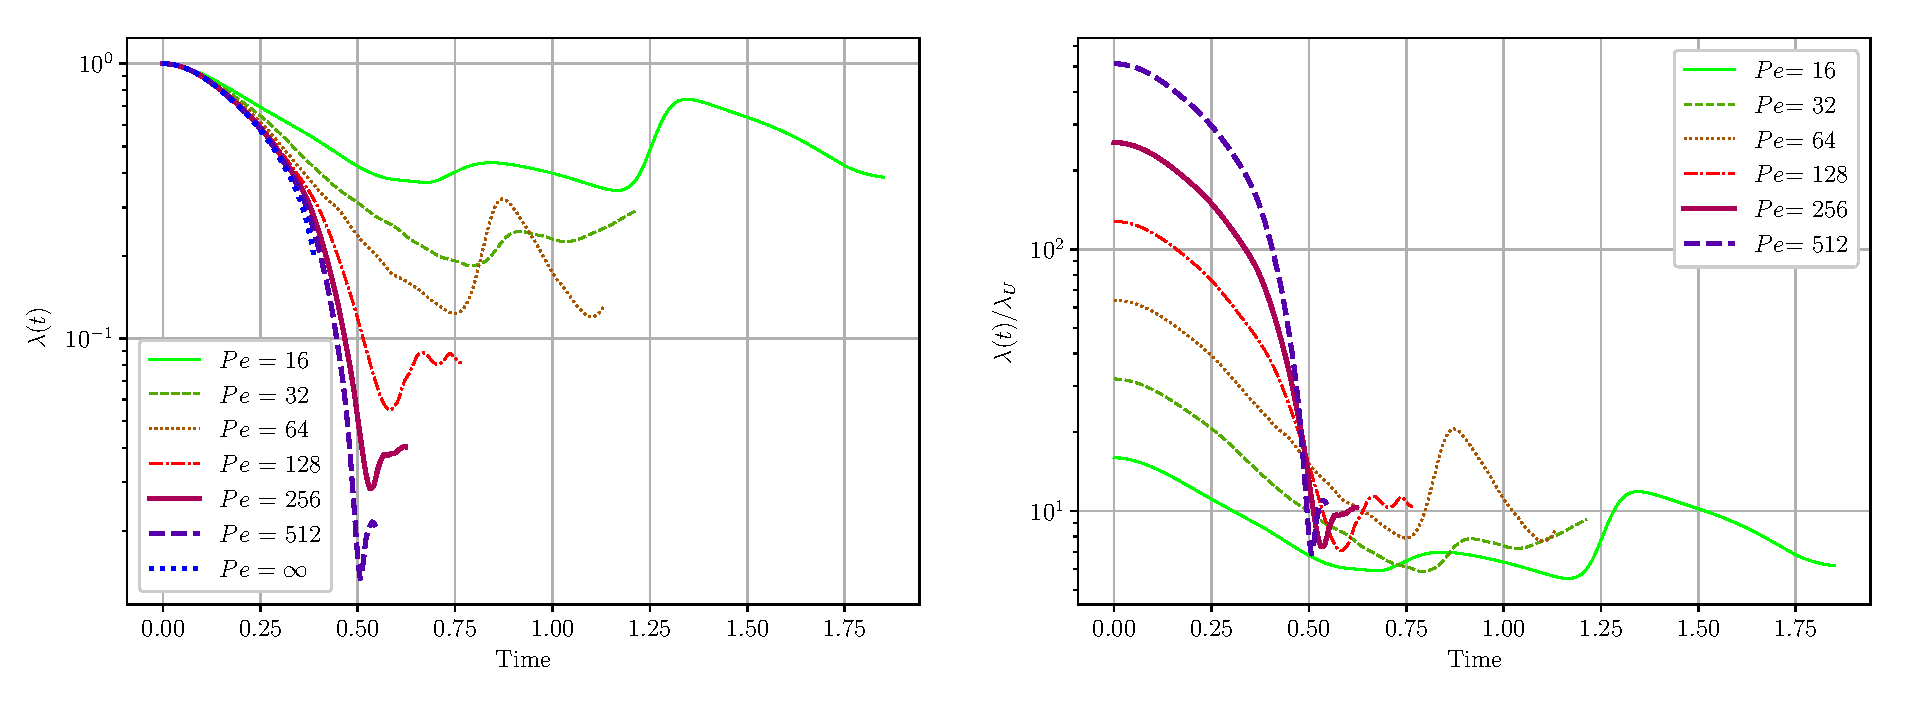
\includegraphics[width=\textwidth]{images/energy_length}
\caption{The left subplot shows the filament length $\lambda$ over time subject to the optimal energy-constrained flow. The right subplot is the same data except scaled: $\lambda(t)/\lambda_{U} = \lambda(t) Pe$.}
\label{fig:energy_length}
\end{figure}
%
\begin{figure}
\centering
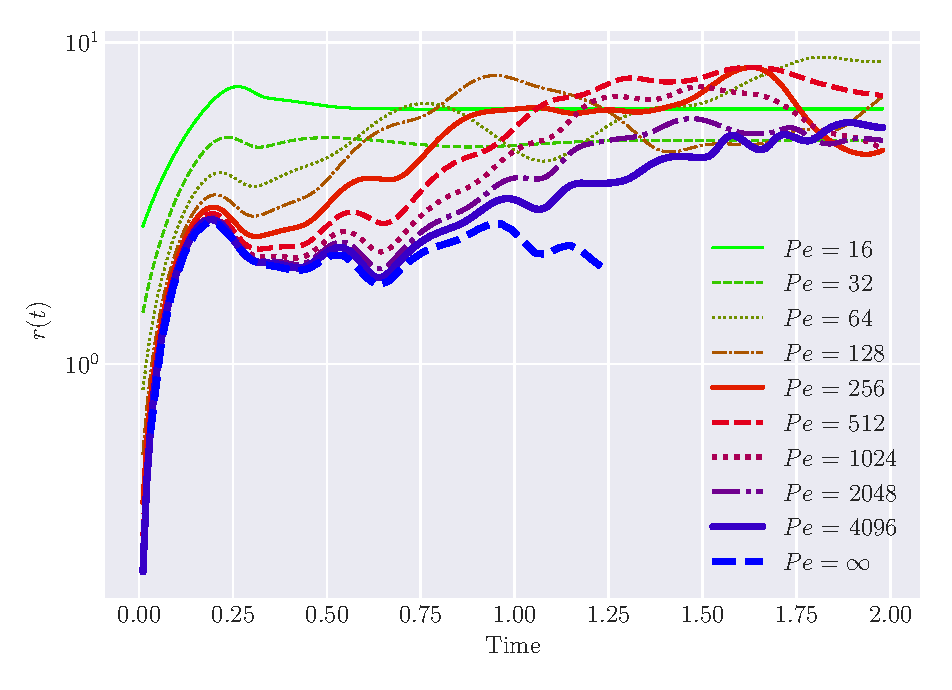
\includegraphics[width=0.5\textwidth]{images/enstrophy_rate}
\caption{Mixing rate $r(t)$ over time when subject to the optimal enstrophy-constrained flow.}
\label{fig:enstrophy_rate}
\end{figure}
%
\begin{figure}
\centering
\includegraphics[width=\textwidth]{images/energy_rate}
\caption{The left subplot shows the mixing rate $r(t)$ over time when subject to the optimal energy-constrained flow. The right subplot is the same data except scaled: $r(t)/r_{U} = r(t)/Pe$.}
\label{fig:energy_rate}
\end{figure}



 Figure \ref{fig:enstrophy_film} shows the evolution of a scalar field under the optimal flow for the enstrophy constraint. The top film strip corresponds to $Pe =\infty$ while the bottom is $Pe = 256$. The time evolution is initially similar but soon diverges over time. Figure \ref{fig:energy_film} shows the evolution for the energy case. The top film strip corresponds to $Pe =\infty$ while the bottom is $Pe = 32$. Notice that, unlike the $Pe = \infty$ cases, the flows with finite $Pe$ are incapable of creating length scales arbitrarily small for either the energy or enstrophy cases.  The left subplot of Figures \ref{fig:enstrophy_length} and \ref{fig:energy_length} shows this phenomena more quantitatively by showing $\lambda$ over time eventually reaching a plateau. The shell-model prediction of this limiting length scale is the Batchelor scale given by $\lambda_{\Gamma} = 1/\sqrt{Pe}$ for the enstrophy case and  $\lambda_{U} = 1/Pe$ for the energy case. The right plots of Figures \ref{fig:enstrophy_length} and \ref{fig:energy_length} shows scaled versions of $\lambda$ given by  $\lambda/\lambda_{\Gamma}$ and $\lambda/\lambda_{U}$ respectively.  Notice how they plateau around an $O(1)$ constant. Thus, this result is consistent with the shell-model predictions. 
   
Figure \ref{fig:enstrophy_rate} shows the mixing rates for the enstrophy case. The rate during the transient phase is $\Gamma$ which is consistent with rates expected from $Pe=\infty$ mixing studies. For all $Pe$ considered, there is an increase in the rate of mixing after transient behaviour has finished to a long-term rate. Surprisingly, this long-term mixing rate appears to be independent of $Pe$ for fixed enstrophy. {\it Thus, this implies that the long-term rate of mixing is only dependent on the rate-of-strain $\Gamma$ and not influenced by the strength of diffusion. }Although, it should be noted that the onset of the long-term rate is affected by the value of $Pe$. When there is strong diffusion (small $Pe$), the Batchelor scale is reached early. From the work of \cite{GI2014} and \cite{CS2013}, $\lambda$ decreases at most exponentially for $Pe = \infty$. If we assume that the local-in-time flows nearly saturate this bound in the transient phase, we model $\lambda$ as  $\lambda (t) = \lambda(0)\exp(- \alpha t) $ during this time. We expect the critical transition time $t_{c}$ that marks the end of this transient period to satisfy $\lambda(t_{c})= \lambda_{\Gamma}$. This time is theorised to be $t_{c}=\frac{1}{\alpha}\ln(\lambda(0)/\lambda_{\Gamma}) = \frac{1}{\alpha}\ln ( \sqrt{Pe} )$ for $Pe>1$ (If $Pe \leq 1$, then there is no transient phase). Hence, a smaller value of $Pe$ will result in an earlier onset of the long-term rate of mixing. Therefore, it is advantageous to have strong diffusion (small $Pe$) so that there is an earlier onset of the long-term mixing rate (although independent of $Pe$) which is an improvement over the mixing rate of the purely non-diffusive situation ($Pe=\infty$).
 
For the energy case, the long-term mixing rate decreases with decreasing $Pe$ (see the left subplot of figure \ref{fig:energy_rate}).  {\it Thus, strong diffusion results in a weak long-term mixing rate}. The right subplot of Figure \ref{fig:energy_rate} is $r/r_{U} =  r/Pe$. We see oscillations of $r/r_{U}$ around a value that is $O(1)$ which indicates that our numerical results are consistent with our predictions from the shell model. Thus, the long-term mixing rate is proportional to $Pe$ in contrast to the long-term mixing rate of enstrophy which carries no dependence on $Pe$. For the enstrophy case, we saw a benefit of picking a lower $Pe$ to result in a earlier onset of the long-term mixing behaviour. The fixed energy case however is different. The onset of the long run-mixing behaviour can be determined by the following model. From the work of \cite{JMP2012} on the fixed energy case, $\lambda(t)$ can decrease linearly in time to produce perfect mixing in finite time. We model the transient phase as $\lambda(t)=\lambda(0)(1-\beta t)$. Therefore, we theorise that the critical transition time is $t_{c}=\frac{1}{\beta}(1 -\lambda_{U}/\lambda(0)) = \frac{1}{\beta}(1 - 1/Pe)$ with $Pe> 1$ (If $Pe \leq 1$, there is not transient phase) for the energy case. Thus, it is true that on can still achieve an earlier onset of the long-term mixing behaviour by choosing a smaller $Pe$. However, an earlier onset time is accompanied by a slower long-term mixing rate. As for choosing a large $Pe$, the onset time is bounded above by $\frac{1}{\beta}$ and results in a faster long-term mixing rate. Thus, it is advantageous to have weak diffusion (large $Pe$) for mixing in the fixed energy case. This benefit is well illustrated by $H^{-1}$ norm in figure \ref{fig:energy_norms}. Notice that the mixing rate is initially slow for $Pe = 512$ but then out competes the mixing rate of smaller values of $Pe$.    



% Figures \ref{fig:enstrophy_norms} and \ref{fig:energy_norms} show the evolution the  $H^{-1}$,  $L^{2}$, and $H^{1}$ norms for different values of finite $Pe$.

\section{Discussion}
\label{sec:discussion}
The local-in-time optimisation results suggest that there is a limiting length scale and rate. The bounds derived, under the $L^{\infty}$ constrained flow assumption, did not result in proving either of these observations. However, they did definitively rule out the possibility of perfect mixing in finite time in either constraint. We believe these bounds could be drastically improved. We surmise that the deficiencies in these bounds is due to not fully exploiting the incompressibility condition. It remains to be shown that $\liminf_{t\rightarrow \infty} \lambda (t)\geq C\lambda_{\Gamma}$ where C is constant dependent on domain and initial condition under an enstrophy constrained flow. A similar problem remains open for the fixed energy case.  If these statements are shown, then many of the results demonstrated here numerically will hold more generally. 

In future work, we would like to consider the optimal control problem coined global-in-time optimisation which tries to minimise the filamentation width at the end time rather than instantaneously attempting to minimise its decay rate. This may lead to flows that are able to extend to even smaller length scales. This global-in-time optimisation has been explored in the work of \cite{Miles2017a} within the context of the shell model. The authors showed that global-in-time and local-in-time optimisation appeared to give similar mixing rates. 


\section{Conclusion}
\label{sec:conclusion}


Our numerical study of local-in-time optimisation suggests that there is a limiting length scale given by a generalised Batchelor length scale which in turn determines a long-term mixing Batchelor rate. Although the Batchelor scale has been a theorised lower bound on the length scales present on turbulent flows, it has not been shown rigorously. We hope this numerical study provides insight and promotes investigation into proving what conditions are necessary on the flow for this to be the case. Furthermore, we showed that these limitations imply that (1), for fixed enstrophy optimal flows, strong diffusion can benefit from an early onset of a long-term mixing rate (where the rate itself however is independent of diffusion strength) while (2), for energy fixed optimal flows, strong diffusion weakens the long-term mixing rate.  


\section*{Acknowledgements}

This work was supported in part by NSF Awards PHY-1205219 and DMS-1515161. One of us (CRD) is additionally grateful for Fellowship funding from the John Simon Guggenheim Memorial Foundation. We are appreciative of the valuable feedback provided by Guatum Iyer, Alexander Kiselev, Ian Tobasco, and Karen Zaya.

 

%Our numerical study of local-in-time optimization suggest that there is a limiting length scale given by $\lambda_{\Gamma} = 1/\sqrt{Pe}$ (in dimensional form, $\sqrt{\kappa/\Gamma}$) for fixed enstrophy and $\lambda_{U} = 1/Pe$ (in dimensional form $\kappa/U$) for fixed energy. The study also suggests a long-term mixing rate given by  $r_{\Gamma} = 1 $ (in dimensional form, $\Gamma$) for fixed enstrophy and $r_{U} = Pe$ (in dimensional form, $U^2/\kappa$) for fixed energy.


%
%Define the spectral variance as
%%
%\begin{equation}
%		\left[ 
%			\frac{\hone{\theta}^2\hmone{\theta}^2}
%			{\ltwo{\theta}^4}  
%			- 1
%		\right].
%\end{equation}
%%
%By using this definition with H\"older's inequality provided that  $\linf{\nabla\vec{u}}\leq \Gamma$, we find that
%%
%\begin{equation}
%\label{eq:length_ineq_rate-of-strain}
%	\ddt{\lambda^2} \geq 2 1/Pe \sigma^2 - 2 \Gamma \lambda^2 .
%\end{equation}
%%
%By taking the long-time average (noted as $\langle \cdot \rangle \equiv\lim_{T\rightarrow\infty}\frac{1}{T}\int_{0}^T \,\, \cdot \,\, dt $ ) of the inequality above, we find that 
%%
%\begin{equation}
%	0 \geq  2 \kappa \tavg{\sigma^2} - 2 \Gamma \tavg{\lambda^2}.
%\end{equation}
%%
%The left hand side is zero since $\lambda^2$ is bounded by Poincar\'e's inequality. Thus, we find that
%%
%\begin{equation}
%	\tavg{\lambda^2} \geq   \lambda_{B}^2 \tavg{\sigma^2} 
%\end{equation}
%%
%where the Batchelor scale is given by $\lambda_{B} = \sqrt{\kappa/\Gamma}.$ 
%
%
%We conclude that ...
%
%By a dimensional analysis, we conjecture that the velocity field with $\hmone{\u}$=1 may be capable decreasing $\lambda$ past the Batchelor scale. 


%\appendix
%\section{Mixing time of modified checkerboard flow}
%\label{appendix:checkerboard}
%We consider a similar  the checkerboard flow from \cite{JMP2012}. Suppose one starts with the initial `binary' dye concentration field where $\theta_{0}(\vec{x}) = 1$ for $x_{1}< 1/2$ and $\theta_{0}(\vec{x}) = -1$ for $x_{1}\geq 1/2$. We constrain $\vec{u}$ to be  $\ltwo{\vec{u}} = 1$. We consider a sheer flow as described by \cite{JMP2012}


%\section{Numerical analysis}
%\label{sec:num_analysis}
%Our conclusions rely heavily on the accuracy of our numerical solutions to the advection diffusion equations. Careful numerical analysis is thus important to make sure the length resolution is sufficient and spectral amplitudes are computed to sufficient numerical accuracy. 


\bibliographystyle{unsrt.bst}
\bibliography{library}




\end{document}